\section{Functionality}
\label{cha:functionality}

The architecture of Kafka consists of several \textbf{servers} and \textbf{clients}. Kafka uses TCP for communication and can be used on any hardware \cite{kafkaDoc}.

Kafka operates as a distributed cluster of \textbf{servers} that can span multiple data centers or cloud platforms. Brokers manage the data storage layer, while Kafka Connect facilitates seamless data exchange between Kafka and other systems. Kafka clusters are designed for mission-critical applications, offering exceptional scalability, fault tolerance, and data integrity \cite{kafkaDoc}.

Kafka \textbf{clients} enable the development of distributed applications and microservices that process event streams efficiently across multiple machines and are resilient to network disruptions or hardware failures. Kafka has built-in clients that are supplemented by an extensive ecosystem of clients provided by the Kafka community. These clients are available for various programming languages, including Java, Scala, Go, Python, C/C++ and even REST APIs \cite{kafkaDoc}.

\subsection{Main Concepts and Terminology}

The central concept of Kafka is the \textbf{event}. Events are notifications that something noteworthy has occured. Kafka's read and write operations are based on these events. An event consists of a key, a value, a timestamp, and optionally, some metadata headers \cite{kafkaDoc}.

An example event looks like this:

\begin{itemize}
    \item Key: "john.doe@example.com"
    \item Value: "Hello World!"
    \item Timestamp: "01.01.1970 00:00:00"
\end{itemize}

\textbf{Producers} are applications that publish events to Kafka, and \textbf{consumers} are applications that subscribe to and process those events. This decoupled architecture enables Kafka to achieve high scalability, as producers and consumers can operate independently, without the need to wait for each other. This flexibility is further enhanced by Kafka's ability to guarantee data integrity, ensuring that events are processed exactly once \cite{kafkaDoc}.

Events are organized and persistently stored within \textbf{topics}. A topic is more or less similar to a folder in a filesystem, with events acting as the files within that folder. For instance, a topic could be named "measurements". Kafka topics are designed to support multiple producers and consumers: a topic can have any number of producers writing events to it, and any number of consumers subscribing to those events. Events within a topic can be read as many times as necessary. Unlike traditional messaging systems, events are not deleted after consumption. Instead, you configure Kafka to retain your events for a specified amount of time, and old events will be discarded after that period. Kafka's performance remains consistent regardless of data size, making it suitable for long-term data storage \cite{kafkaDoc}.

As illustrated in Figure \ref{fig:partitions}, to enhance scalability and parallelism, Kafka \textbf{partitions} topics into multiple "buckets" distributed across different brokers. This allows multiple consumers and producers to read and write the topic simultaneously to take advantage of the distributed nature of the Kafka cluster. When a new event is published to a topic, it is appended to one of the corresponding partitions. Additionally, events with the same key are written to the same partition, ensuring data consistency and enabling efficient retrieval based on the key. Kafka maintains the order of events within each partition, ensuring that messages are read in the same sequence they were stored \cite{kafkaDoc}.

\begin{figure}[ht]
    \centering
    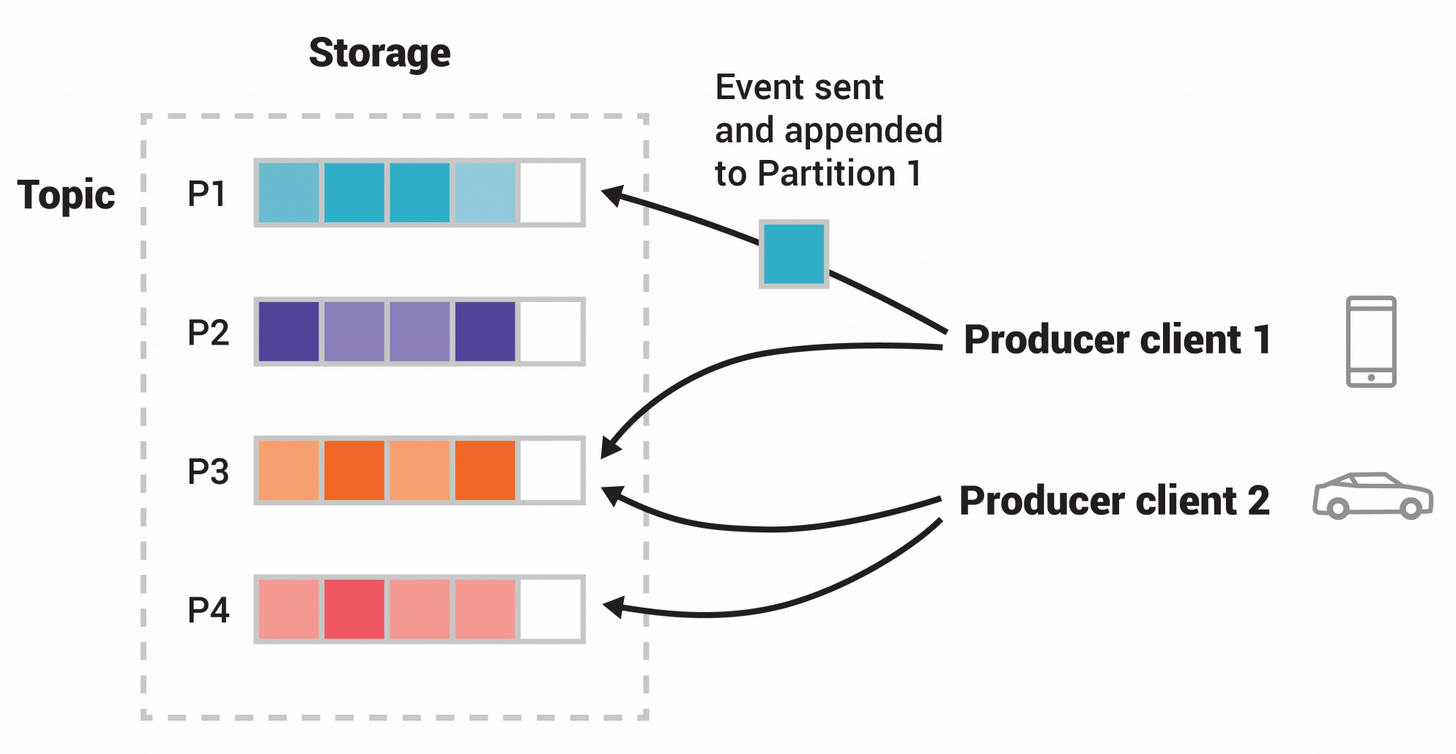
\includegraphics[width=8.5cm]{images/partitions.png}
    \caption{This topic consists of four partitions (P1-P4). Two producers are independently publishing events to the topic, with events with similar keys being grouped into the same partition. Both producers may write to the same partition if necessary \cite{kafkaDoc}.}
    \label{fig:partitions}
\end{figure}

To ensure that data remains accessible even if a broker fails or requires maintenance, each topic can be \textbf{replicated} across multiple brokers. The replication factor of 3 is a common setting that helps to maintain data availability and fault tolerance. Each partition has a partition leader that processes all read and write requests for this partition. The followers of the partition replicate the leader. If the leader fails, a follower becomes the new leader. The leaders are evenly distributed across the cluster, which means that each broker is the leader of several partitions \cite{kafkaDoc}.

\subsection{Architectural Overview}

Figure \ref{fig:architecture} provides a comprehensive overview of the architecture and functionality of Kafka. A major change in the latest versions is the introduction of KRaft as a consensus protocol, replacing Apache ZooKeeper. This change enables Kafka to manage its metadata independently, eliminating the need for external coordination. As a result, Kafka gains self-sufficiency and increased resilience while benefiting from improved scalability and performance \cite{kull2023secure}.

\begin{figure}[ht]
    \centering
    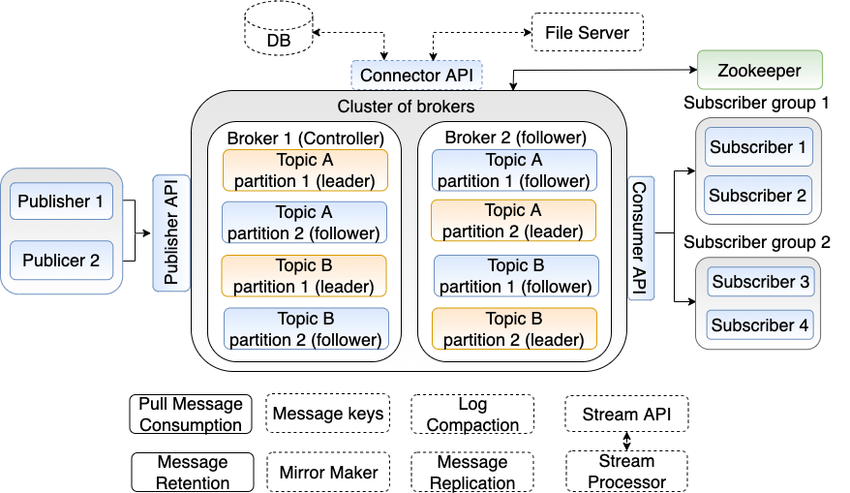
\includegraphics[width=8.5cm]{images/architecture.png}
    \caption{Apache Kafka architecture with mandatory and optional services \cite{lazidis2022publish}.}
    \label{fig:architecture}
\end{figure}